\documentclass[11pt]{amsbook}
\usepackage[utf8]{inputenc}
\usepackage{../HBSuerDemir}
\usepackage{tikz}
\usetikzlibrary{arrows}
\date{October 2016}

\begin{document}

\hPage{b1p1/25}


\section { Intervals }

    Some subsets of \hSoR, denoted by $[a, b]$, $(a, b)$, $[a, b)$, $(a, b]$ and called \underline{intervals}, are of particular importance. Their definitions as well as their graphs on the number axis are given below:
    
    \begin{enumerate}
        \item $\hPairingCurly{x: a \leq x\leq b} = [a, b]$ 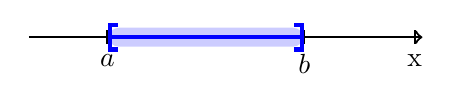
\begin{tikzpicture}[scale=5]
            \draw[->, thick] (0,0) -- (1,0);
            \foreach \x/\xtext in {0.2/$a$,0.7/$b$,0.98/x}
                \draw[thick] (\x,0.5pt) -- (\x,-0.5pt) node[below] {\xtext};
            \draw[[-, ultra thick, blue] (0.2,0) -- (0.7,0);
            \draw[{-]}, ultra thick, blue] (0.2,0) -- (0.7,0);
            \fill[opacity = 0.2, blue,rounded corners=1ex] (0.2,-.16ex) -- (0.7, -.16ex) -- (0.7, .16ex) -- (0.2,.16ex) -- cycle;
            \end{tikzpicture}

        \item $\hPairingCurly{x: a < x < b} = (a, b)$ 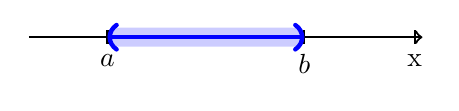
\begin{tikzpicture}[scale=5]
            \draw[->, thick] (0,0) -- (1,0);
            \foreach \x/\xtext in {0.2/$a$,0.7/$b$,0.98/x}
                \draw[thick] (\x,0.5pt) -- (\x,-0.5pt) node[below] {\xtext};
            \draw[(-, ultra thick, blue] (0.2,0) -- (0.7,0);
            \draw[-), ultra thick, blue] (0.2,0) -- (0.7,0);
            \fill[opacity = 0.2, blue,rounded corners=1ex] (0.2,-.16ex) -- (0.7, -.16ex) -- (0.7, .16ex) -- (0.2,.16ex) -- cycle;
            \end{tikzpicture}

        \item $\hPairingCurly{x: a \leq x < b} = [a, b)$ 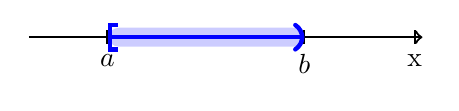
\begin{tikzpicture}[scale=5]
            \draw[->, thick] (0,0) -- (1,0);
            \foreach \x/\xtext in {0.2/$a$,0.7/$b$,0.98/x}
                \draw[thick] (\x,0.5pt) -- (\x,-0.5pt) node[below] {\xtext};
            \draw[[-, ultra thick, blue] (0.2,0) -- (0.7,0);
            \draw[-), ultra thick, blue] (0.2,0) -- (0.7,0);
            \fill[opacity = 0.2, blue,rounded corners=1ex] (0.2,-.16ex) -- (0.7, -.16ex) -- (0.7, .16ex) -- (0.2,.16ex) -- cycle;
            \end{tikzpicture}

        \item $\hPairingCurly{x: a < x\leq b} = (a, b]$ 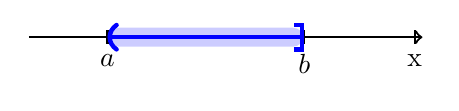
\begin{tikzpicture}[scale=5]
            \draw[->, thick] (0,0) -- (1,0);
            \foreach \x/\xtext in {0.2/$a$,0.7/$b$,0.98/x}
                \draw[thick] (\x,0.5pt) -- (\x,-0.5pt) node[below] {\xtext};
            \draw[(-, ultra thick, blue] (0.2,0) -- (0.7,0);
            \draw[{-]}, ultra thick, blue] (0.2,0) -- (0.7,0);
            \fill[opacity = 0.2, blue,rounded corners=1ex] (0.2,-.16ex) -- (0.7, -.16ex) -- (0.7, .16ex) -- (0.2,.16ex) -- cycle;
            \end{tikzpicture}

        \item $\hPairingCurly{x: x \leq c} = (-\infty, c]$ 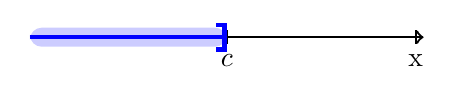
\begin{tikzpicture}[scale=5]
            \draw[->, thick] (0,0) -- (1,0);
            \foreach \x/\xtext in {0.5/$c$,0.98/x}
                \draw[thick] (\x,0.5pt) -- (\x,-0.5pt) node[below] {\xtext};
            %\draw[[-, ultra thick, blue] (0,0) -- (0.5,0);
            \draw[{-]}, ultra thick, blue] (0,0) -- (0.5,0);
            \fill[opacity = 0.2, blue,rounded corners=1ex] (0.0,-.16ex) -- (0.5, -.16ex) -- (0.5, .16ex) -- (0.0,.16ex) -- cycle;
            \end{tikzpicture}

        \item $\hPairingCurly{x: x < c} = (-\infty, c)$ 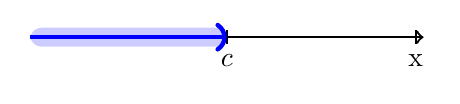
\begin{tikzpicture}[scale=5]
            \draw[->, thick] (0,0) -- (1,0);
            \foreach \x/\xtext in {0.5/$c$,0.98/x}
                \draw[thick] (\x,0.5pt) -- (\x,-0.5pt) node[below] {\xtext};
            %\draw[[-, ultra thick, blue] (0,0) -- (0.5,0);
            \draw[-), ultra thick, blue] (0,0) -- (0.5,0);
            \fill[opacity = 0.2, blue,rounded corners=1ex] (0.0,-.16ex) -- (0.5, -.16ex) -- (0.5, .16ex) -- (0.0,.16ex) -- cycle;
            \end{tikzpicture}
            
        \item $\hPairingCurly{x: d \leq x} = [d , \infty)$ 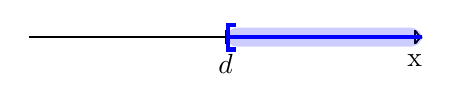
\begin{tikzpicture}[scale=5]
            \draw[->, thick] (0,0) -- (1,0);
            \foreach \x/\xtext in {0.5/$d$,0.98/x}
                \draw[thick] (\x,0.5pt) -- (\x,-0.5pt) node[below] {\xtext};
            \draw[[-, ultra thick, blue] (0.5,0) -- (1,0);
            %\draw[{-]}, ultra thick, blue] (0,0) -- (0.5,0);
            \fill[opacity = 0.2, blue,rounded corners=1ex] (0.5,.16ex) -- (1.0, .16ex) -- (1.0, -.16ex) -- (0.5,-.16ex) -- cycle;
            \end{tikzpicture}
            
        \item $\hPairingCurly{x: d < x} = (d , \infty)$ 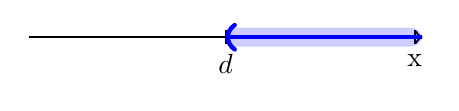
\begin{tikzpicture}[scale=5]
            \draw[->, thick] (0,0) -- (1,0);
            \foreach \x/\xtext in {0.5/$d$,0.98/x}
                \draw[thick] (\x,0.5pt) -- (\x,-0.5pt) node[below] {\xtext};
            \draw[(-, ultra thick, blue] (0.5,0) -- (1,0);
            %\draw[{-]}, ultra thick, blue] (0,0) -- (0.5,0);
            \fill[opacity = 0.2, blue,rounded corners=1ex] (0.5,.16ex) -- (1.0, .16ex) -- (1.0, -.16ex) -- (0.5,-.16ex) -- cycle;
            \end{tikzpicture}     
            
        \item $\hPairingCurly{x: all x} = (-\infty , \infty) = \hSoR$ 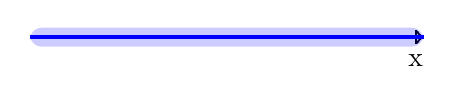
\begin{tikzpicture}[scale=5]
            \draw[->, thick] (0,0) -- (1,0);
            \foreach \x/\xtext in {0.98/x}
                \draw[thick] (\x,0.5pt) -- (\x,-0.5pt) node[below] {\xtext};
            \draw[, ultra thick, blue] (0.0,0) -- (1,0);
            %\draw[{-]}, ultra thick, blue] (0,0) -- (0.5,0);
            \fill[opacity = 0.2, blue,rounded corners=1ex] (0.0,.16ex) -- (1.0, .16ex) -- (1.0, -.16ex) -- (0.0,-.16ex) -- cycle;
            \end{tikzpicture}
    \end{enumerate}
    
    The interval $[a, b]$, representing a line segment as its graph on the x-axis and including the end points $a, b$ is called a \underline{closed intervals} which reduces to a single point in case the end points coincide.
    
    The interval $(a, b)$ is distinguished from [a,b] by not containing the end points a, b and accordingly is called an \underline{open intervals} and reduces therefore to the empty set $\emptyset$ when $a = b: (a,a) = \emptyset$.
    
    The intervals $[a, b)$ and $(a, b]$ being closed at one end open at the other are referred to as \underline{semi open} or \underline{semi closed intervals}.
    
    The remaining\footnote{I have changed the word "remaing" to "remaining"} intervals in the list are expressed by the use of symbols $-\infty$ and $\infty$ called respectively \underline{minus infinity} and \underline{plus infinity}. It is important to note that they are not numbers, but are convenient symbols for denoting points at in-\footnote{The whole word is "infinity"}
    


\end{document}
